
\begin{figure*}
	\centering
	\subfloat[Conference-name tag cloud]{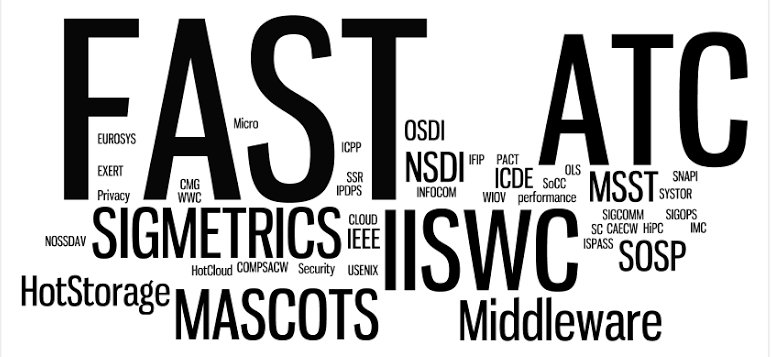
\includegraphics[scale=0.25]{presyn-figures/conference-names-wordle.jpg}} \hfill
	\subfloat[Year-of-publication tag cloud]{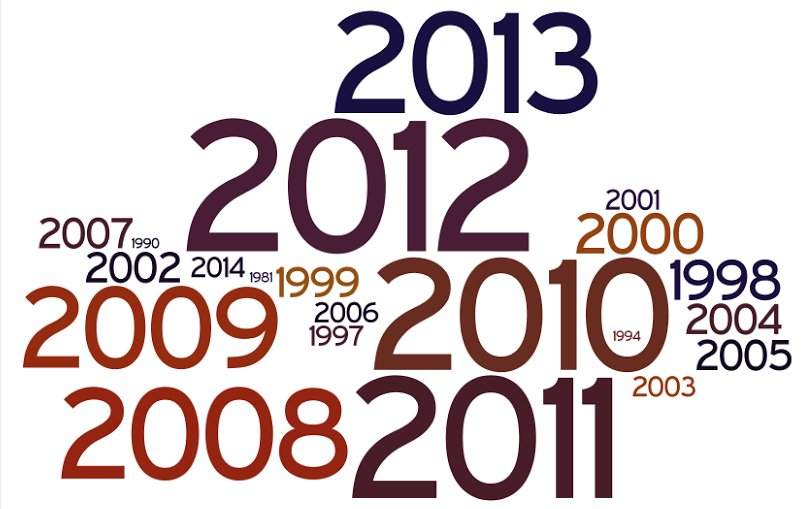
\includegraphics[scale=0.25]{presyn-figures/year-of-publication-wordle.jpg}}
	\\
	\caption{Representation of the conferences and the years of publication covered in our survey}
	\label{fig:tag-clouds}
\end{figure*}


%In the course of the dataset survey, 
We surveyed the datasets used in over
100 publications amounting to a total of over 350 datasets. A similar survey
for storage deduplication datasets (covering 120 datasets from 33 research 
papers) is presented in \cite{generating-datasets}, wherein the requirements
specified for such datasets is that they should be realistic, 
sufficiently large, as well as easily accessible/distributed to 
other researchers. 

The paper \cite{generating-datasets} does not
mention by name which publications were surveyed by the authors, except for 
stating that the 33 research papers were from top conferences from the
years 2010 and 2011. Due to such limited information available, we 
undertook the survey all over again, while at the same time not restricting
ourselves to only a couple of years\textemdash{}instead, we cast a wider net for our
survey by including all papers that were related to any of the following
topics:- (i)~Storage deduplication\index{Storage deduplication}, 
(ii)~Memory deduplication\index{Memory deduplication}, 
(iii)~Storage characterization, and 
(iv)~I/O characterization.


Since the number of papers considered in our survey is huge (more than 100),
instead of listing out the conference names and the year of publication, we
present the following tag clouds (refer Fig.~\ref{fig:tag-clouds}(a) and (b))
which are meant to represent the survey\index{Survey} 
coverage. As can be seen from the
tagcloud in Fig.~\ref{fig:tag-clouds}(a), our survey covers the
important conferences in the areas of storage and workload characterization,
namely \textbf{FAST}, \textbf{ATC}, \textbf{SIGMETRICS} and \textbf{IISWC},
to name a few. Moreover, the years of publication (refer 
Fig.~\ref{fig:tag-clouds}(b)) for the surveyed papers
are mostly within 2009 to 2014, with a few lying even beyond as well.
With this wide coverage of conferences and years of publication, we are
positive that we have covered the necessary ground for this survey.

As mentioned earlier, we classify
the dataset surveyed into two sets (i)~\textit{Public datasets} and
(ii)~\textit{Proprietary datasets}, and for each of these sets, we 
need to distinguish the dataset further based on whether they are one of 
the following:
\begin{enumerate}
	\item I/O traces with content representation, 
	\item I/O traces without content representation,
	\item Storage metadata\index{Metadata} with content representation, or
	\item Storage metadata without content representation
\end{enumerate}
The first item in the above list is the kind of trace we are looking for,
i.e. I/O activity traces with content representation. However, we found
that almost all of the public datasets available online fall in one of 
the other three categories listed above.

\subsection{Public dataset repositories}\index{Dataset repositories}
By the term \textit{public datasets}, we allude to those datasets or 
traces that have 
been made available online by the respective owners. 
A popular repository for
storage and I/O traces is the SNIA-IOTTA Repository~\cite{snia-iotta-repo} which 
is a collection of traces from multiple publications maintained under
the Storage Network Industry Association's Input/Output Traces, Tools and 
Analysis Technical Work Group. Another popular repository
is the one maintained by HP Labs~\cite{hplabs-repo} which 
contains many tools and benchmarks as well, in addition to traces. 
Note that, there are several other small repositories, each hosting the traces 
or datasets for a single or few publications, we list them separately in 
the next section under \textit{Public individual datasets}.
Below we provide a listing of those online trace repositories, 
which contain huge number of traces (i.e. multiple trace sets, not just one)
and are available to the researchers for development and analysis of network 
and storage systems.
\begin{enumerate}
	\item \textbf{SNIA IOTTA Repository}~\cite{snia-iotta-repo}: collaborative effort under SNIA IOTTA TWG to provide storage-related I/O traces, tools and analysis to the entire research community free of cost.
	\item \textbf{HP Labs Repository}~\cite{hplabs-repo}: provides several file system and application traces captured using HP Labs' tools like DataSeries and Lintel. However, some of these traces are very old, and may not be representative of current systems.
	\item \textbf{UMass Trace Repository}~\cite{umass-repo}: provides network, storage, and other traces, some of which are generated at UMass while some others are donated.
	\item \textbf{Internet Traffic Archive}~\cite{ita-repo}: provides access to traces of Internet network traffic. 
	\item \textbf{VMware image repository}~\cite{thoughtpolice-repo}: provides many VMware images with various Linux distributions installed like CentOS, Debian, Fedora, FreeBSD and OpenSUSE.
	%\item FSL labs repository
	%\item LiveDFS repo?
\end{enumerate}

Next, we discuss the suitability of the traces, hosted at 
each of the above public dataset repositories, 
for the purpose of I/O deduplication evaluation.

\subsubsection{1. SNIA IOTTA Repository traces}
This repository contains several trace sets including Block I/O traces, NFS 
traces and System call traces. The publications that make use of these 
traces are~\cite{flexi-replay, iodedup, animation-nfs, winservers, metadata-evolution, tracefs}, among which \cite{iodedup} is the only paper which deals
with I/O deduplication-related traces\textemdash{}none of the other trace sets at
this repository have data content representation, and hence they are not
suitable for evaluating I/O deduplication techniques.

\subsubsection{2. HP Labs Repository traces}
This repository contains several file system and application traces, however
some of these traces are very old, and also none of these traces have any
content representation either.

\subsubsection{3. UMass Trace Repository traces}
This repository provides traces for network, storage, memory, etc and is a 
collection of traces used in various publications like~\cite{flexi-replay, 
intradisk-parallelism, memorybuddies}. Apart from the traces provided 
of memory contents, none of the other traces in this repository has any
content representation. Moreover, the memory traces are also published 
as snapshots of memory contents and not in the form of an I/O trace, 
indicative of which block is being inserted or evicted from cache at 
which time. Hence, even these traces are not suitable for evaluation of
I/O deduplication techniques.

\subsubsection{4. Internet Traffic Archive traces}
This repository provides access to traces of Internet network traffic, for
potential characterization, benchmark generation, etc and even though
a few of these traces (eg. LBL-TCP-3, LBL-PKT) are packet traces, instead
of just web requests or HTTP traces, however they still do not represent
the packet content or payload. Hence, none of these traces are suitable
for I/O deduplication analysis, not even as synthetic workloads.

\subsubsection{5. VMware image repository}
This is a repository of 78 VMware virtual machine images with various
Linux distributions installed in the default configuration. This 
repository has been used in a few publications~\cite{p-dedupe, ddelta} to
motivate storage deduplication and compression. However, since these
are static images and not I/O workloads in themselves, they are not
suitable for evaluation of I/O deduplication techniques.

\subsection{Public individual datasets}
\begin{enumerate}
	\item \textbf{I/O deduplication traces}~\cite{iodedup-online}: Traces provided by the I/O deduplication paper~\cite{iodedup} which we also used in our evaluation
	\item \textbf{Plan 9 traces}~\cite{p9-traces}: File system snapshots of the Plan 9 file system deployed in the Computing Sciences Research center of Bell Labs. Has content representation, but is suitable only for storage deduplication studies, not for I/O deduplication
	\item \textbf{Animation-bear dataset}~\cite{animation-bear}: Traces released by HP Labs, collected at a feature animation company\textemdash{}these are NFS traces and have no content representation
	\item \textbf{Linux kernel \& GCC sources}~\cite{kernel-src, gcc-src}: A few papers~\cite{p-dedupe, ddelta} use kernel and GCC sources to perform study of storage deduplication systems, by exploiting the fact that multiple successive versions of the same software tend to have a lot of overlapping content.
\end{enumerate}

These are individual datasets that were used for the 
characterization and evaluation in a couple of papers
and have been made available online for use by other researchers.
Among these, the first dataset (i.e. the I/O deduplication traces at~\cite{iodedup-online})
is the one we have used for DRIVE evaluation in the previous chapter. This
traces are also present at the SNIA IOTTA repository mentioned above, and 
is the only I/O access trace which has content representation included.
The remaining traces are all either storage metadata traces or I/O traces
without content representation, hence unfit for evaluation of I/O deduplication
techniques.

\begin{table} [t]
	\begin{tabular}{|l|l|c|c|c|l|} \hline
	\textbf{No.} & \textbf{Dataset} & \textbf{Cited} & \textbf{Related to} & \textbf{Comments regarding} \\
	\textbf{} & \textbf{source} & \textbf{by} & \textbf{I/O, storage} & \textbf{suitability for} \\
	\textbf{} & \textbf{} & \textbf{} & \textbf{or memory} & \textbf{I/O dedup evaluation} \\ \hline
	1 & IODEDUP traces & \cite{iodedup} & I/O & Suitable for I/O dedup evaluation \\ 
	2 & SNIA IOTTA Repo & \cite{flexi-replay, winservers, metadata-evolution, tracefs} & I/O & No content representation \\ 
	3 & HP Labs Repo & \cite{storage-system-security, hplabs-repo} & Storage, I/O & No content representation \\
	4 & UMass Trace Repo & \cite{flexi-replay, intradisk-parallelism, memorybuddies} & Storage, I/O & No content representation \\
	5 & Internet Traffic Archive & \cite{failure-of-poisson, search-for-invariants, ita-repo} & Internet & No content representation \\
	6 & VMware Image Repo & \cite{p-dedupe, ddelta} & Storage & Storage metadata, not I/O \\
	7 & Plan 9 traces & \cite{venti} & Storage & Storage metadata, not I/O \\
	8 & Animation-bear dataset & \cite{animation-bear} & I/O & No content representation \\ 
	9 & Kernel \& GCC source & \cite{p-dedupe, ddelta} & Storage & Storage metadata, not I/O \\ \hline
	\end{tabular}
	\caption{Summary of \textit{public} datasets uncovered in the survey}
	\label{tab:public-listed}
\end{table}

\subsection{Proprietary datasets}\index{Proprietary datasets}
So far we have seen the publicly-available storage and I/O datasets. However,
this is a small fraction of all the datasets that have been used and cited
in all the papers that we surveyed. In other words, most of the datasets that
are used for evaluation in literature are rarely hosted 
publicly~\cite{generating-datasets} or made
available to other researchers for further perusal and analysis. In what
follows, we present a brief categorization of such datasets and cite the
works which have used each category of dataset.

\begin{enumerate}
 \item \textit{Homes:} This basically consists of the home directories of 
 several employees or students or researchers hosted on a common or 
 shared storage. The access workload is such that the files are read
 and written by a single user each, although the user may end up 
 making several copies of the same file for purposes of editing, 
 translations, conversions, versioning, etc. Such datasets are used
 in~\cite{primary-data-dedup, backup-workloads-characterization, 
 datadomain, cifs-study, redundancy-alternatives}.
 \item \textit{WebServer:} Consists of traces (storage or I/O) from
 webserver workloads, and includes Web ``search'' workloads also in some
 cases. Such workloads are traced and characterized in several research 
 efforts like~\cite{storagecharacterization, filesystem-workloads, 
 content-sampling, my-cache-or-yours, filesize-distrib-cause, 
 web-cable-modem, scaling-phenomena, web-client-access-patterns}.
 \item \textit{CollaborationShares:} This consists of shared storage
 among a group of researchers or collaborators such that the files
 are created by one user and accessed by many others for read and/or
 updates. This dataset may also have duplicates due to multiple 
 copies for editing and versioning~\cite{content-sampling, idedup, 
 cifs-study, redundancy-alternatives}
 \item \textit{SoftwareDeployment:} This consists of the data from 
 a server which contains VM images, softwares and binaries to be 
 used for deployment by users, and the workload is such that the
 files are created by one or more system administrators and used
 or accessed by a bigger user population. This dataset may have duplicates due
 to similarities across the softwares and/or VM images~\cite{similarity}.
 Such datasets are used for the evaluation of storage deduplication
 in \cite{idedup, redundancy-alternatives}.
 \item \textit{VM-Dataset:} A set of a few hundred VM images with
 installations of different versions of operating systems, applications
 and libraries is considered under this dataset. The similarities
 across VM images are due to multiple VM images being instantiated
 from a single golden master or template image~\cite{similarity, dedup-effectiveness, 
 primary-data-dedup, vdn, building-highperf-dedup}.
 \item \textit{VM-Backup:} This consists of a setup where one or more VMs
 are fully or partially backed up regularly, such
 that the backups would have lot of redundancies amongst them~\cite{ddelta, 
 vmdk-backups, hysteresis-rechunking, lowcost-dedup-for-backup}.
 \item \textit{DatabaseBackup:} Similar to the VM-Backup dataset mentioned above,
 several works also use database backup workloads for evaluation
 of storage deduplication techniques~\cite{ddelta, backup-workloads-characterization, 
	 hybrid-dedup, ventana}. 
\end{enumerate}

\begin{table} [t]
	\begin{tabular}{|l|l|c|l|} \hline
		\textbf{No.} & \textbf{Dataset category} & \textbf{Dataset description} & \textbf{Cited by} \\ \hline
1 & \textit{Homes} & Home directories on shared storage & \cite{primary-data-dedup, backup-workloads-characterization, datadomain, cifs-study, redundancy-alternatives} \\ 
2 & \textit{WebServer} & Traces from webserver workloads & \cite{filesystem-workloads, content-sampling, web-cable-modem, scaling-phenomena, web-client-access-patterns} \\
3 & \textit{CollaborationShares} & Files created by one, read by many & \cite{idedup, cifs-study, redundancy-alternatives, content-sampling} \\
4 & \textit{SoftwareDeployment} & Files created by one, used by many & \cite{idedup, primary-data-dedup, redundancy-alternatives} \\
5 & \textit{VM-Dataset} & Few hundred VM images & \cite{similarity, vdn, primary-data-dedup, dedup-effectiveness, building-highperf-dedup} \\
6 & \textit{VM-Backup} & Full or partial backup of VMs& \cite{ddelta, vmdk-backups, hysteresis-rechunking, lowcost-dedup-for-backup} \\
7 & \textit{DatabaseBackup} & Backup of production databases & \cite{ddelta, backup-workloads-characterization, hybrid-dedup, ventana} \\ \hline
	\end{tabular}
	\caption{Summary of \textit{proprietary} datasets uncovered in the survey}
	\label{tab:proprietary-listed}
\end{table}

We summarize the results of our above dataset survey in 
Table~\ref{tab:public-listed} for \textit{publicly-available} datasets
and in Table~\ref{tab:proprietary-listed} for \textit{proprietary} datasets. 
For each dataset, we identify 
it by a name, and list a few representative reference
papers in which the dataset has been utilized. For each dataset,
we also mention whether it is related to I/O, storage
or memory traces and present comments regarding the dataset's
suitability for use in evaluation of I/O deduplication techniques.

\subsection{Benchmarks}
Some benchmarking\index{Benchmarking} 
tools and application benchmarks have also been used for
workload generation\index{Workload generation} in literature. 
Some of the most popular benchmarks
for Storage I/O workload generation are as under:-
\begin{enumerate}
	\item \textbf{Filebench}~\cite{filebench}: It is a file 
		system and storage 
	      benchmark that can generate both micro and macro workloads. 
	      It allows detailed workload specification using Workload
	      Model Language (WML) as well. It includes several popular
	      macro-workloads like web server, mail server and database 
	      server.
	\item \textbf{dbench}~\cite{dbench}: This tool can be used to stress test
	      a storage system to figure out its saturation performance
	      level. It allows complex load specification, however the
	      point is not to just generate specific load levels, rather
	      the point is to push the storage system to its limits for
	      the purpose of benchmarking its performance.
	\item \textbf{HiBench}~\cite{hibench}: This is a benchmark suite
	      for Hadoop mapreduce application benchmarking,
	      comprising of both micro-benchmarks as well as application
	      workloads like web search, machine learning and analytic
	      querying.
	\item \textbf{IOzone}~\cite{iozone}: This is a file system benchmark
	      tool that generates and measures the performance of a wide
	      variety of file system operations like \texttt{read}, \texttt{write},
	      \texttt{re-read}, \texttt{re-write}, \texttt{random read},
	      \texttt{mmap} and so on.
	\item \textbf{IOMeter}~\cite{iometer}: This is a load generation and
	      characterization tool for both storage and network, and can
	      generate loads on single or multiple systems.
	\item \textbf{PostMark}~\cite{postmark}: This is a benchmark to 
	      emulate and measure the functionality of email servers, 
		  web servers and news servers.
	\item \textbf{FIO}~\cite{fio}: Flexible IO tester (FIO) is a tool that 
		  allows the user to write a job file according to the load that 
		  needs to be simulated, and the tool spawns multiple processes
		  to generate the requested load.
	\item \textbf{CloudSuite}~\cite{cloudsuite}: CloudSuite is a benchmark
		  suite currently consisting of 8 application benchmarks that are
		  based on real-world setups in today's datacenters. The benchmarks
		  supported include data serving, data caching, web serving 
		  benchmarks and so on.
	\item \textbf{TPC Benchmarks}~\cite{tpc}: The Transaction Processing
		Performance Council (TPC) defines benchmarks related to transaction
		processing and databases, which can be used to benchmark the 
		performance of various applications, like OLTP, decision support
		and many more.
	\item \textbf{SPEC Benchmarks}~\cite{spec}: The Standard Performance 
		Evaluation Corporation (SPEC) establishes, maintains and endorses
		a standardized set of benchmarks for high-performance computers,
		like compute-intensive benchmarks, mail server benchmarks (now retired),
		virtualization performance benchmarks, etc.
	\item \textbf{NAS Parallel Benchmarks}~\cite{nasa}: This is a suite of
		programs designed to evaluate parallel supercomputers, at the
		NASA Advanced Supercomputing Division.
	\item \textbf{HPC Challenge Benchmark}~\cite{hpcc}: This is a benchmark
		suite comprising of 7 tests, measuring various metrics like rate of memory
		operations sustainable, total communication capacity of the network,
		latency and bandwidth of simultaneous communications, etc.
	\item \textbf{PARSEC}~\cite{parsec}: The Princeton Application Repository for 
		Shared-Memory Computers (PARSEC) is a benchmark suite containing many
		multi-threaded programs simulating diverse workloads, like image
		processing, financial analytics, and video encoding.
	\item \textbf{Kernel}~\cite{kernel-src} \textbf{and other sources}~\cite{am-utils, emacs} \textbf{compile benchmark}
\end{enumerate}		

Most of the above benchmarks are either too simplistic or have so many 
control knobs that it is a daunting task to choose the correct 
settings~\cite{generating-datasets}. For example, the work in 
\cite{storage-benchmark-coverage} shows that to exhaustively try all
settings in the benchmarks like FIO, IOzone and Postmark is too time
consuming\textemdash{}instead, 
it recommends that only the minimum and maximum
value for every setting need be tested. It makes an arguable assumption 
that the intermediate settings will result in output that lies between
the outputs for the minimum and maximum settings.

Given any benchmarking tool which has several knobs that can be tweaked,
we might still try tweaking the knobs exhaustively to determine those
settings which produce a compatible workload for 
I/O deduplication evaluation.
However, the onus of proving that the resulting tweaked workload is a 
realistic workload\index{Realistic workload} would still loom large. 
Particularly, most of these benchmarks
do not have realistic content representation~\cite{dedis}, 
and generate either highly duplicate (eg. Bonnie++~\cite{bonnie}) 
or highly random content (eg. 
PostMark~\cite{postmark}, Fstress~\cite{fstress}).
We thus make the claim that,
after having established the initial worth of the DRIVE system using
the available traces, there is nothing more to be gained by evaluation
using synthetic benchmarks\index{Synthetic benchmarks}. 
Further evaluation of the DRIVE system is
valuable only if performed using real-world workloads 
or using ``realistic'' benchmarks.

A study of various benchmarks and analysis by ``benchmarking'' of the
benchmarks is done in~\cite{rocket-science}, which shows that most of
the literature consists of researchers using their own customized
or \textit{ad-hoc}
synthetic benchmarks, which results in incomparable results across
papers. This is an undesirable situation, 
and the work in \cite{rocket-science}
proposes that there should first be a consensus regarding the
dimensions to be benchmarked, and then agreement on the methodology
to benchmark each dimension and comparison of results across systems.
It proposes several dimensions for file system benchmarking, like 
\textit{I/O, on-disk, metadata, caching} and \textit{scaling}.
Due to lack of consensus regarding dimensions, and
the unsuitability of most existing benchmarks for IO deduplication
evaluation, we turn to characterizing the available traces instead.


%\begin{figure*}
%	\centering
%	\includegraphics[scale=0.25]{presyn-figures/datasets-classified.pdf}
%	\caption{Classification of publicly-available datasets: \textit{Only one 
%	set of traces falls in the category we are interested in, which is I/O 
%	traces with content representation}}
%	\label{fig:datasets-classified}
%\end{figure*}


\subsection{Summary of survey findings}
The purpose of this survey is to find publicly-available datasets
of I/O traces with content representation. Our survey revealed that
among the publicly-available datasets, only the ones available 
via IODEDUP paper~\cite{iodedup} have content representation,
and we have already used them for our evaluation in the previous
chapter. All other publicly-available datasets lie in one of
the other three categories.
%, as depicted in Fig.~\ref{fig:datasets-classified}.

Based on our findings that (i) existing public datasets are not
relevant for evaluation of I/O deduplication, (ii) many relevant
datasets are proprietary and not publicly-available, as well as,
(iii) existing benchmarks are not ``realistic'' enough for our purposes, 
we turn to the next avenue of using real-world traces to build
synthetic traces ourselves. We performed a detailed literature
survey of this area (i.e., generating realistic traces) and
find that all such efforts rely on trace characterization of some 
available real-world traces, to generate realistic synthetic traces. 
Therefore, next we perform trace characterization of the 
available \textit{homes} and \textit{webvm} traces,
which may be helpful to build realistic synthetic traces in future.
